%%%%%%%%%%%%%%%%%%%%%%%%%%%%%%%%%%%%%%%%%
% APA Assignment Article
% LaTeX Template
% Version 2.0 (February 7, 2023)
%
% This template originates from:
% https://www.LaTeXTemplates.com
%
% Author:
% Vel (vel@latextemplates.com)
%
% License:
% CC BY-NC-SA 4.0 (https://creativecommons.org/licenses/by-nc-sa/4.0/)
%
% NOTE: The bibliography needs to be compiled using the biber engine.
%
%%%%%%%%%%%%%%%%%%%%%%%%%%%%%%%%%%%%%%%%%

%----------------------------------------------------------------------------------------
%	PACKAGES AND OTHER DOCUMENT CONFIGURATIONS
%----------------------------------------------------------------------------------------

\documentclass[
	letterpaper, % Paper size, use either a4paper or letterpaper
	10pt, % Default font size, can also use 11pt or 12pt, although this is not recommended
	unnumberedsections, % Comment to enable section numbering
	twoside, % Two side traditional mode where headers and footers change between odd and even pages, comment this option to make them fixed
]{APAAssignment}

\addbibresource{bibliography.bib} % BibLaTeX bibliography file

\runninghead{MICS CYBER 252, Fall-2024 Hands On Lab 2} % A shortened article title to appear in the running head, leave this command empty for no running head

\footertext{\textit{Hands On Lab 2 (2.5.2)  } (MICS CYBER 252, Fall -2024)} % Text to appear in the footer, leave this command empty for no footer text

\setcounter{page}{1} % The page number of the first page, set this to a higher number if the article is to be part of an issue or larger work

%----------------------------------------------------------------------------------------
%	TITLE SECTION
%----------------------------------------------------------------------------------------

\usepackage[title,toc,titletoc]{appendix}
\usepackage{titlesec}
\usepackage{lscape}
\usepackage{fontawesome}

\title{Hands-On lab 2 \\ MICS-252, Fall 2024} % Article title, use manual lines breaks (\\) to beautify the layout

% Authors are listed in a comma-separated list with superscript numbers indicating affiliations
% \thanks{} is used for any text that should be placed in a footnote on the first page, such as the corresponding author's email, journal acceptance dates, a copyright/license notice, keywords, etc
% Affiliations are output in the \date{} command
\date{UC Berkleley School of Information \\
MICS Course 252 Fall 2024 (Kristy Westphal)
}


\author{
	Prepared by: Karl-Johan Westhoff \\
	email: \href{mailto:kjwesthoff@berkeley.edu}{kjwesthoff@berkeley.edu}
}


% % Full-width abstract
% \renewcommand{\maketitlehookd}{%
% 	\begin{abstract}
% 		\noindent Lorem ipsum dolor sit amet,rta porttitor.
% 	\end{abstract}
% }

%----------------------------------------------------------------------------------------

\setcounter{tocdepth}{5}
\setcounter{secnumdepth}{5}
\usepackage[title]{appendix}

\begin{document}
\onecolumn
\maketitle % Output the title section

%----------------------------------------------------------------------------------------
%	ARTICLE CONTENTS
%----------------------------------------------------------------------------------------

\section{Introduction}
Introduction Here
I extensively used the walkthroughs in \cite{CycubicsDocsWebGoat}

\section{Lessons Learned}
LL Here
Reset password exercise is nefarious


\section{Topics for Further Exploration}
Topics Here

JWT token exploitation


\subsection{Open source and supply chain vulnerabilities}
Library dependencies and open source
Log4j
tar.xz
openssh

Comment:
Some organizations prefer to have 'someone to blame' and if they paid for proprietary software they feel that they can unload some liability.


\section{Conclusion}
Conclusion Here

%----------------------------------------------------------------------------------------
%	 REFERENCES
%----------------------------------------------------------------------------------------
\clearpage
\printbibliography % Output the bibliography

%----------------------------------------------------------------------------------------



%----------------------------------------------------------------------------------------
%	 Appendices
%----------------------------------------------------------------------------------------

\appendix


\clearpage
\chapter{Appendices}
\begin{appendices}


%\hypertarget{webgoat-setup}{%

\section{Identity and Authentication Failure}}\label{app:AuthAndFailure}
\subsection{Authentication Bypass}
There is  a bug in the password reset system, changing the names in the http POST payload solves the assignment   

\begin{figure}[!ht] % Single column figure
	\centering
	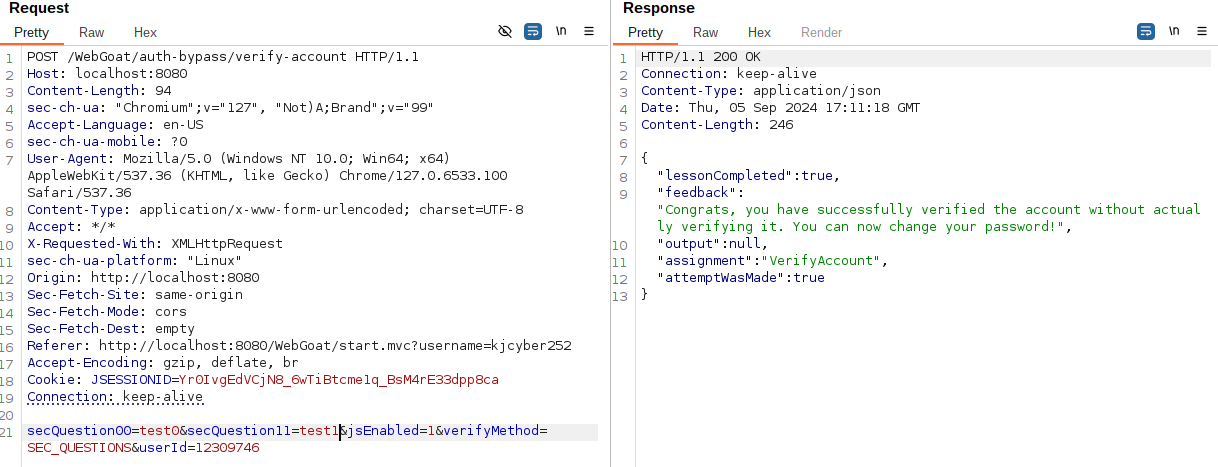
\includegraphics[width=\linewidth]{IdentAndAuthBypass.png}
	\caption{Authentication reset bypassed by changing the secQuestion names the POST request payload}
	\label{fig:app:AuthBypass}
\end{figure}

\subsection{Insecure Login}
For some reason some credentials are hardcoded or left from previous logins when sending the POST request empty.

\begin{figure}[!ht] % Single column figure
	\centering
	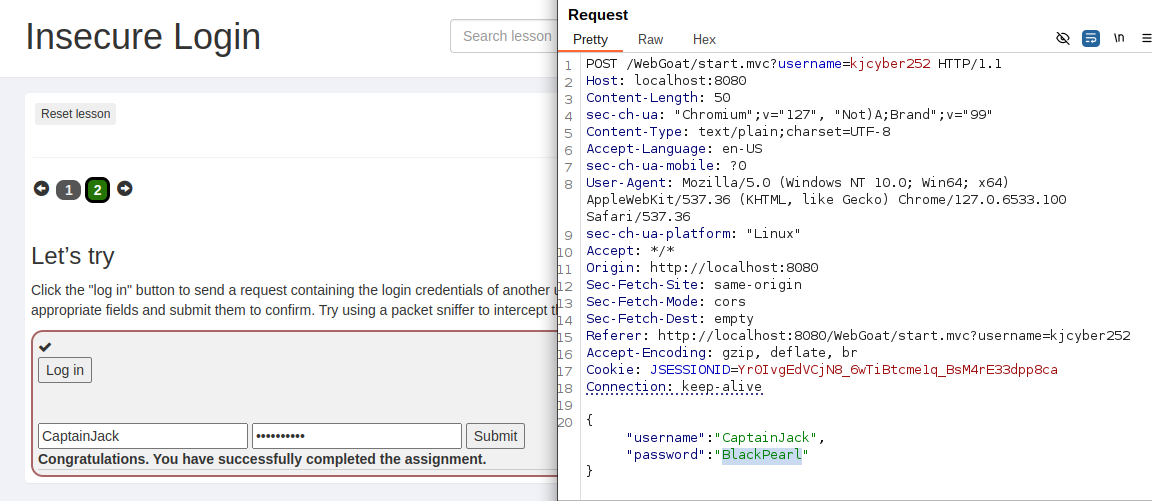
\includegraphics[width=\linewidth]{InsecureLogin.png}
	\caption{Captain Jacks credentials in the POST}
	\label{fig:app:InsecureLogin}
\end{figure}

\subsection{JWT Tokens}
JWT tokens are sometimes used in place of authentication cookies, i.e. without the cross reference protections the browser offers. JWT's are basically ways to send information verified by signatures. In this case the header can be manipulated not to do the verification and blindly trust the token.

\subsubsection{JWT(4)}
Decoded the token on jwt.io and found 'user'

\subsubsecion{JWT(6)}
Decoded and manipulated the token using Burps Decoder , setting the signature alg to 'none' and admin to true and got "something" accepted 202

\begin{figure}[!ht] % Single column figure
	\centering
	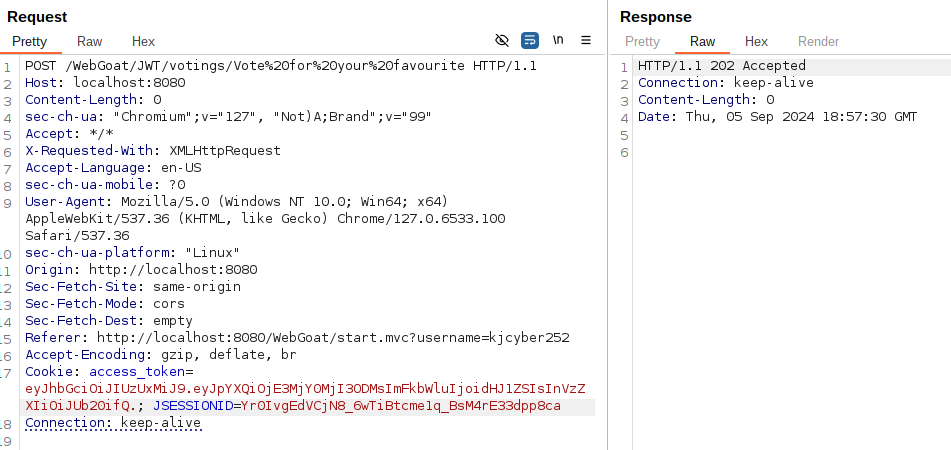
\includegraphics[width=\linewidth]{JWT6.png}
	\caption{JWT token manipulations}
	\label{fig:app:JWT6}
\end{figure}

\subsubsecion{JWT(8)}
I was unable to load the Quiz..


\subsubsecion{JWT(11)}
JWT Cracking


\subsubsection{JWT(13) Refresh Tokens}
Manipulated the token by setting the algorithm to 'none' and manipulating the expiation

\begin{figure}[!ht] % Single column figure
	\centering
	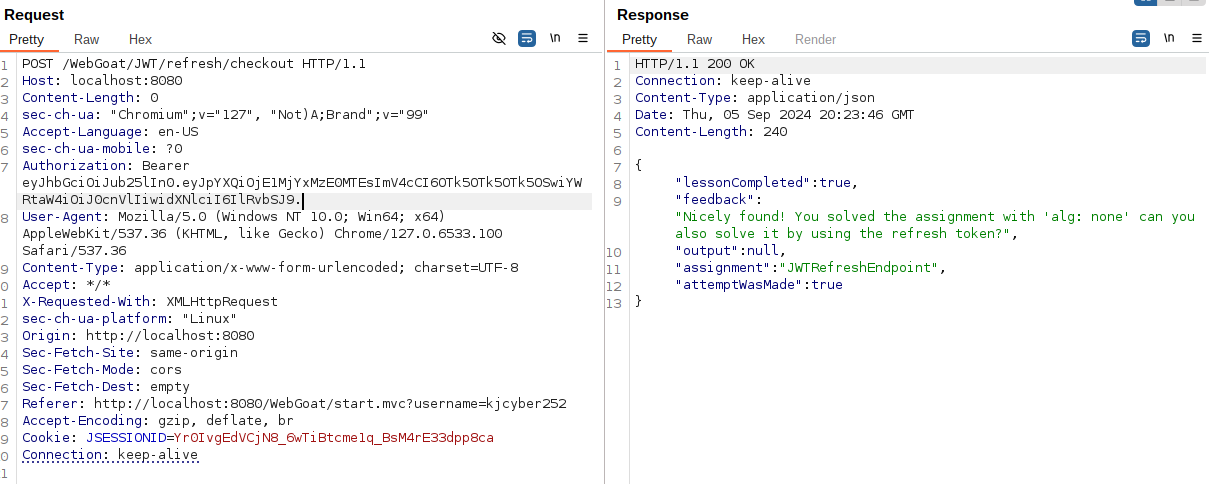
\includegraphics[width=\linewidth]{JWT13_1.png}
	\caption{JWT token manipulations, without refresh.. see next}
	\label{fig:app:JWT13}
\end{figure}


\subsubsection{JWT(16/18) Avanced Token generation..}
I found this one difficult and relied on a walkthrough from \cite{MediumJWT8}, where references to the WebGoat source code was used to solve the assignment.

\begin{figure}[!ht] % Single column figure
	\centering
	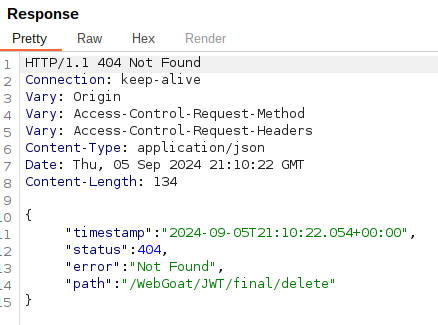
\includegraphics[width=0.25\linewidth]{JWT16_404.png}
	\caption{Could not find the "/WebGoat/JWT/final/delete" endpoint turns out the right page is in 18}
	\label{fig:app:JWT16}
\end{figure}

Manipulated the jwt from the delete POST by changing the names to tom, manipulating expiration and changing the 'kid' to: 
\begin{verbatim}
	"something_else' UNION SELECT 'bmV3X2tleQ==' FROM INFORMATION_SCHEMA.SYSTEM_USERS; --", 
\end{verbatim}

All signed with "new\_key": giving:

\begin{figure}[!ht] % Single column figure
	\centering
	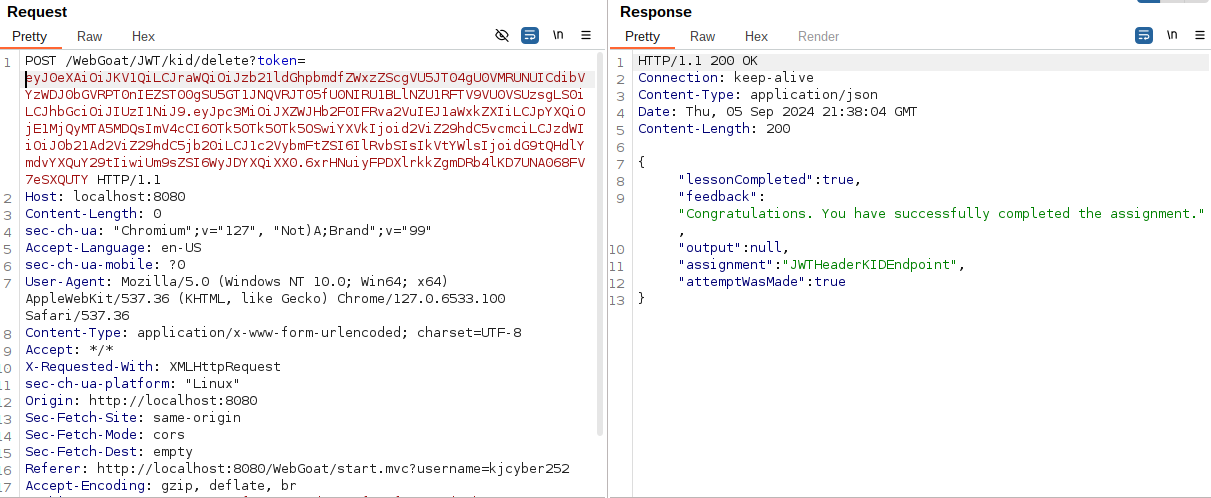
\includegraphics[width=1\linewidth]{JWT_18.png}
	\caption{/WebGoat/JWT/final/delete" Solved!}
	\label{fig:app:JWT18}
\end{figure}

\subsection{Password reset}

\subsubsection{Password Reset 2: Email functionality with WebWolf}

\begin{figure}[!ht] % Single column figure
	\centering
	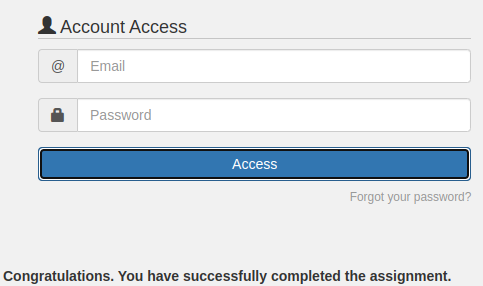
\includegraphics[width=0.5\linewidth]{pw_reset_2.png}
	\caption{Basic password functionality working}
	\label{fig:app:pw_reset_2}
\end{figure}

\subsubsection{Password Reset 4: Security questions}

\begin{figure}[!ht] % Single column figure
	\centering
	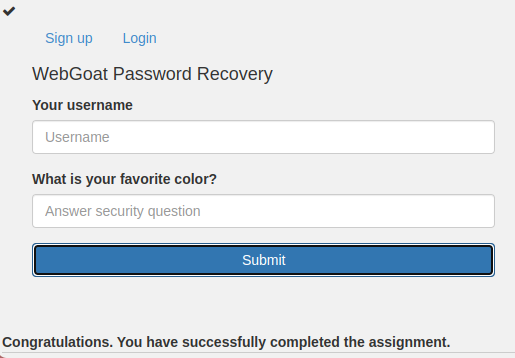
\includegraphics[width=0.5\linewidth]{pw_reset_4.png}
	\caption{Reset challenge questions brute force-able, un:Top, pw:purple (from \cite{CycubicsDocsWebGoat}}
	\label{fig:app:pw_reset_4}
\end{figure}

\subsubsection{Password Reset 5: The Problem with Security Questions}
Will be sure not to implement.


\subsubsection{Password Reset 6: Creating the password reset link}
Redirecting the reset password link, i  





\section{Vuln. and Outdated Components}\label{app:VulnAndOutdatedComponents}
\subsection{(5)The exploit is not always in "your" code}\label{app:VulnAndOutdatedComponents5}

\begin{figure}[!ht] % Single column figure
	\centering
	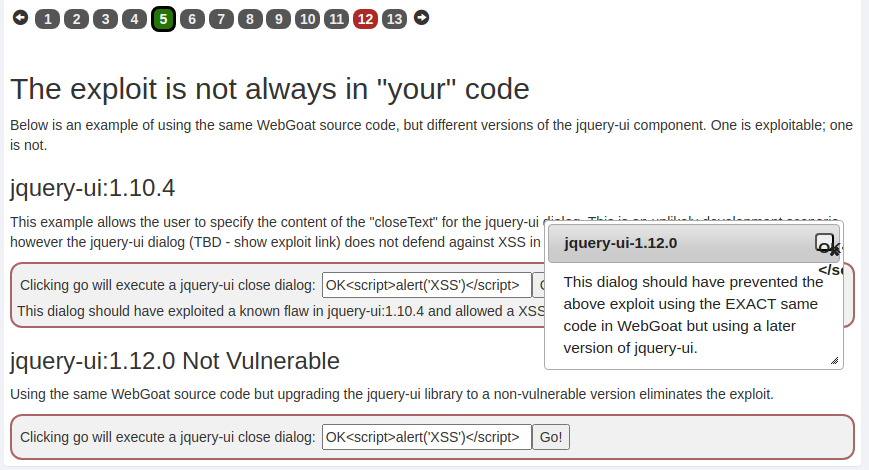
\includegraphics[width=\linewidth]{VulnComponents5.png}
	\caption{Differences in JQuery versions, one of which is vulnerable to reflected XSS }
	\label{fig:app:vuln5}
\end{figure}

\subsection{(12)Exploiting CVE-2013-7285 (XStream)}\label{app:VulnAndOutdatedComponents12}
This one is scary. XStream is a serial/de-serializer for XML, JSON etc. when used as a deserializer, it opens up possibility of an OS command injection resulting in remote code execution. XStream.fromXML deserializes into an Java Object, vulnerable to OS injection as <interface>org.owasp.webgoat.lessons.vulnerablecomponents.Contact</interface> the Contact function will be executed   

\begin{figure}[!ht] % Single column figure
	\centering
	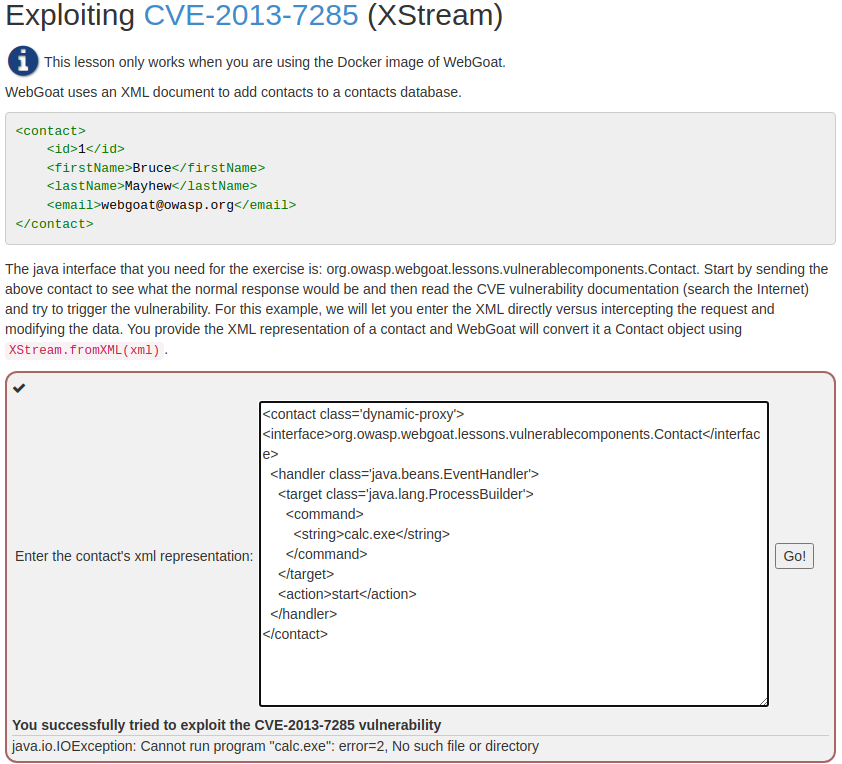
\includegraphics[width=\linewidth]{VulnComponents12.png}
	\caption{XStream deserializes and executes Contact function resulting in remote code execution}
	\label{fig:app:vuln12}
\end{figure}


\begin{figure}[!ht] % Single column figure
	\centering
	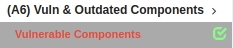
\includegraphics[width=0.3\linewidth]{VulnOutdatedSolved.png}
	\caption{Section A6 Solved}
	\label{fig:app:vulnSolved}
\end{figure}

\section{Security Logging Failures and Client Side}\label{app:SecurityLogging}



\section{Client Side}\label{app:ClientSide}

% \begin{figure}[!ht] % Single column figure
% 	\includegraphics[width=\linewidth]{Pasted image 20240823155542.png}
% 	\caption{Docker Desktop}
% 	\label{fig:Docker-Desktop}
% \end{figure}




\end{appendices}
\end{document}
